\documentclass{article}
\usepackage{graphicx}
\usepackage{subcaption}

% to make table of contents clickable
\usepackage{hyperref}
\hypersetup{
}

\author{CD}
\title{DD}

\begin{document}

\thispagestyle{empty} % to hide pagenum
\begin{center}

	\vspace{3cm}

	\large $\bf Software$ $\bf Engineering$ $\bf 2$

  
\includegraphics[width=\linewidth]{../RASD/images/polimi-logo.png}
  \vspace{2cm}
  

  \Huge $\bf SafeStreets$


	\huge $\bf Design$  $\bf Document$

	\vspace{1cm}

  Authors:
	\vspace{1cm}
	\begin{tabular}{r|l}
		 Federico Cazzola & \large mat 945835\\
		 Francesco Dotti & \large mat 945232\\
	\end{tabular}

	\vspace{1cm}

  Professor: Di Nitto Elisabetta
	
	\vspace{3cm}
  \normalsize Academic Year 2019-2020

	\vspace{2mm}
	\small Version 1.0

\end{center}

\newpage

\thispagestyle{empty} % to hide pagenum
\tableofcontents

\newpage
  
\section{Introduction}
\subsection{Purpose}
The purpose of this document is to describe how the system will be built, giving specific and technical details about architectural and design decisions. Also implementation, integration and testing plans will be discussed.
In particular the document presents:
\begin{itemize}
	\item The SafeStreet System architecture (its parts and how they interact)
	\item The runtime behavior
	\item The design patterns
	\item User Interfaces
	\item Implementation, integration and testing plans 
\end{itemize}

\subsection{Scope}
The scope of the Safestreets project, as already specified in the RASD, is to give the user the possibility to report traffic violation, in particular, parking violation (eg. parking in a spot reserved for disabled people, parking in an helicopter pitch, parking on the sidewalk). The system will allow the users to select the type of violation leading to differt amount of ticket value.
The system will help the authorities to identify more infractions and therefore to issue more tickets which should increase the attention and respect of the citizens regarding the traffic rules.
Furthermore thanks to the increased number of ticket the municipality will have more money to invest in the community. This extra money could be used to do some interventions following the suggestions provided by SafeStreets.

\subsection{Definitions, Acronyms, Abbreviations}
\subsubsection{Definitions}
% \begin{itemize}
% \end{itemize}

\subsubsection{Acronyms}
\begin{itemize}
	\item \textbf{RASD}: Requirements Analysis and Specifications Document  
	\item \textbf{DD}: Design Document
\end{itemize}

\subsubsection{Abbreviations}
% \begin{itemize}
% \end{itemize}

\subsection{Revision history}
\begin{itemize}
	\item Version 1.0 | First Release
\end{itemize}

\subsection{Reference Documents}
\begin{itemize}
	\item Specification document: “SafeStreets Mandatory Project Assignment” 	
	\item \href{https://www.uml-diagrams.org}{UML diagrams}
	\item IEEE Standard for Information Technology—Systems Design—Software Design Descriptions (IEEE Std 1016TM-2009)
\end{itemize}

\subsection{Document Structure}
\begin{itemize}
	\item Chapter 1 is the introduction.
	\item Chapter 2 provides details about the system architecture, its components and how they interact.
	\item Chapter 3 describes the UX and shows the user interface providing mockups.
	\item Chapter 4 describes how the requirements ( defined in the RASD ) are mapped to the design elements defined in this document.
	\item Chapter 5 presents the implementation, integration and test plan. It shows how the different components of the application are integrated with each other and how they react. Also the testing strategies are described and the risks in the application are analyzed.
	\item Chapter 6 shows the effort spent by each group member
\end{itemize}

\section{Architectural design}
\subsection{Overview: High-level components and their interaction}
The	application to be developed is a distributed application and the three logic software layers of Presentation (P), that manages the user interaction with the system, Application (A), that handles the business logic of the application and its functionalities, and Data access (D), that manages the information with access to the database, are thought to be divided on three different hardware layers (tiers) that represent a machine (or a group of machines), so that any logic layer has, in principle, its own dedicated hardware: we have a so called three-tier architecture.
This architecture is thought to guarantee to the system characteristics of scalability and flexibility and to lighten the server side splitting it into two nodes. In particular, the second tier is thought to contain only the business logic to physically separate clients and data to guarantee more safety in accessing to data since the system deals with sensitive data. 
The following image show the high-level architecture of the system without providing any detail through the ArchiMate modeling language that is lighter than the UML language for such a simple 
representation.
\begin{figure}[ht]
\centering
	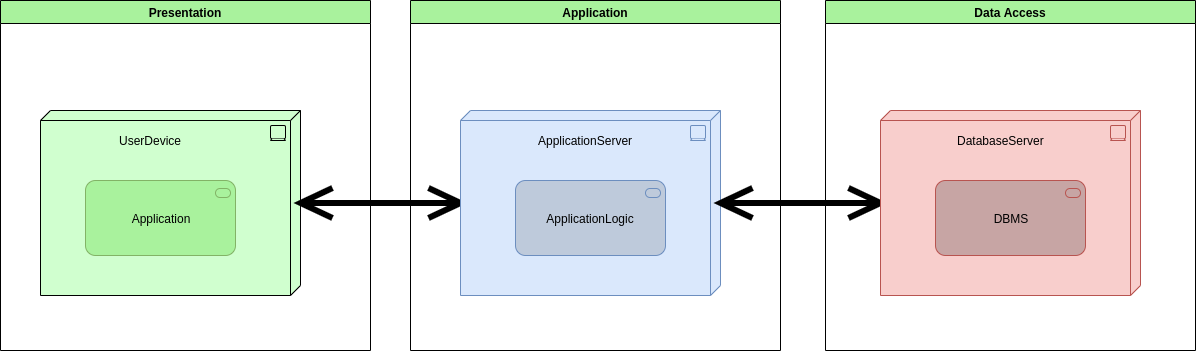
\includegraphics[width=1.0\textwidth]{images/tier-structore.png}
	\caption{Tier Structure}
	\label{fig:tier-structore}
\end{figure}
\subsection{Component view}
\subsection{Deployment view}
\subsection{Runtime view}
\subsection{Component interfaces}
\subsection{Selected architectural styles and patterns}
\subsection{Other design decisions}

\section{User interface design}

\section{Requirements traceability}

\section{Implementation, integration and test plan}

\section{Effort spent}
	\begin{center}
		{\bf Cazzola Federico \href{https://github.com/f-cazzola}{@f-cazzola} }
		\vspace{2mm}

			\begin{tabular}{p{1.3cm}|p{1.8cm}|p{6.7cm}}
				\hline
				\bf Date & \bf \makebox[1.8cm][c]{Hours} & \bf \makebox[6.7cm][c]{Description} \\
				23/11/19 & \makebox[1.8cm][c]{2} & \makebox[6.7cm][c]{Architectural design}\\
				\hline
				total    & \makebox[1.8cm][c]{2}
			\end{tabular}
	\end{center}
	\vspace{1cm}

	\begin{center}
		{\bf Dotti Francesco \href{https://github.com/dottif}{@dottif} }
		\vspace{2mm}

			\begin{tabular}{p{1.3cm}|p{1.8cm}|p{6.7cm}}
				\hline
				\bf Date & \bf \makebox[1.8cm][c]{Hours} & \bf \makebox[6.7cm][c]{Description} \\
				\hline
				15/11/19 & \makebox[1.8cm][c]{1} & \makebox[6.7cm][c]{Initial Structure}\\
				22/11/19 & \makebox[1.8cm][c]{1.5} & \makebox[6.7cm][c]{Introduction}\\
				total    & \makebox[1.8cm][c]{2.5}
			\end{tabular}
	\end{center}

\end{document}
